\chapter{Géométrie dans l'espace}

\section{Les solides usuels}

\subsection{Les solides droits}

\begin{prop}[Volume d'un solide droit]

	Le volume d'un solide est noté $\mathcal{V}$.

	\begin{itemize}
		\item Le volume d'un \textbf{cube} de côté $c$ est :
		      \[
			      \mathcal{V} = c \times c \times c = c^3
		      \]

		\item Le volume d'un \textbf{parallélépipède rectangle} de longueur $L$, de largeur $\ell$ et de hauteur $H$ est :
		      \[
			      \mathcal{V} = L \times \ell \times H
		      \]

		\item Le volume d'un \textbf{cylindre} ou d'un \textbf{prisme} droit de hauteur $H$ est
		      \[
			      \mathcal{V} = \text{Aire de la base} \times H
		      \]
	\end{itemize}
	\begin{center}
		~\hfill
		\begin{tikzpicture}[x={(1cm,0cm)}, y={(0.5cm,0.3cm)}, z={(0cm,1cm)}, scale=0.8]
			\draw[bleu, thick] (0,0,0) -- (2,0,0) -- (2,0,2) -- (0,0,2) -- cycle;
			\draw[bleu, thick] (0,0,2) -- (0,2,2) -- (2,2,2) -- (2,0,2);
			\draw[bleu, thick] (2,0,0) -- (2,2,0) -- (2,2,2);
			\draw[bleu, dashed] (0,0,0) -- (0,2,0) -- (2,2,0);
			\draw[bleu, dashed] (0,2,0) -- (0,2,2);
			\node[below] at (1,0,0) {$c$};
			\node[anchor=north, font=\small, gris] at (current bounding box.south) {Cube};
		\end{tikzpicture}
		\hfill
		\begin{tikzpicture}[x={(1cm,0cm)}, y={(0.5cm,0.3cm)}, z={(0cm,1cm)}, scale=0.8]
			\draw[bleu, thick] (0,0,0) -- (3,0,0) -- (3,0,1.6) -- (0,0,1.6) -- cycle;
			\draw[bleu, thick] (0,0,1.6) -- (0,2,1.6) -- (3,2,1.6) -- (3,0,1.6);
			\draw[bleu, thick] (3,0,0) -- (3,2,0) -- (3,2,1.6);
			\draw[bleu, dashed] (0,0,0) -- (0,2,0) -- (3,2,0);
			\draw[bleu, dashed] (0,2,0) -- (0,2,1.6);
			\node[below] at (1.5,0,0) {$L$};
			\node[right] at (3,1,-0.1) {$\ell$};
			\node[left] at (0,0,0.8) {$H$};
			\node[anchor=north, font=\small, gris] at (current bounding box.south) {Parallélépipède rectangle};
		\end{tikzpicture}
		\hfill
		\begin{tikzpicture}[scale=0.8]
			\fill[vert!30] (0,0) ellipse (1 and 0.3);
			\draw[bleu, thick] (0,2) ellipse (1 and 0.3);
			\draw[bleu, thick] (-1,2) -- (-1,0) arc[start angle=180, end angle=360, x radius=1, y radius=0.3] -- (1,2);
			\draw[bleu, dashed] (-1,0) arc[start angle=180, end angle=0, x radius=1, y radius=0.3];
			\draw[rouge, <->] (1.4,0) -- (1.4,2) node[midway, right] {$H$};
			\node[anchor=north, font=\small, gris] at (current bounding box.south) {Cylindre};
		\end{tikzpicture}
		\hfill
		\begin{tikzpicture}[x={(1cm,0cm)}, y={(0.5cm,0.3cm)}, z={(0cm,1cm)}, scale=0.8]
			\fill[vert!30] (0,0,0) -- (2.4,0,0) -- (1,1.8,0) -- cycle;
			\draw[bleu, thick] (0,0,0) -- (2.4,0,0) -- (2.4,0,2) -- (0,0,2) -- cycle;
			\draw[bleu, thick] (0,0,2) -- (1,1.8,2) -- (2.4,0,2);
			\draw[bleu, dashed] (0,0,0) -- (1,1.8,0) -- (2.4,0,0);
			\draw[bleu, dashed] (1,1.8,0) -- (1,1.8,2);
			\draw[bleu, thick] (2.4,0,0) -- (2.4,0,2);
			\draw[rouge, <->] (2.9,0,0) -- (2.9,0,2) node[midway, right] {$H$};
			\node[anchor=north, font=\small, gris] at (current bounding box.south) {Prisme droit};
		\end{tikzpicture}
		\hfill~
	\end{center}
\end{prop}

\begin{ex}
	\nline
	\begin{itemize}
		\item Un parallélépipède rectangle de longueur $5\,\text{cm}$, de largeur $3\,\text{cm}$ et de hauteur $2\,\text{cm}$ a pour volume :
		      \[
			      \mathcal{V} = 5 \times 3 \times 2 = 30\,\text{cm}^3
		      \]

		\item Un cylindre de hauteur $5\,\text{cm}$, dont la base est un disque de rayon $3\,\text{cm}$, a pour volume :
		      \[
			      \mathcal{V} = \pi \times 3^2 \times 5 = 45\pi\,\text{cm}^3 \approx 141{,}4\,\text{cm}^3
		      \]
	\end{itemize}
\end{ex}

\subsection{Pyramide et cône}

\begin{prop}[Volume d'une pyramide, d'un cône]
	\nline
	\begin{center}
		\begin{tikzpicture}[x={(1cm,0cm)}, y={(0.5cm,0.3cm)}, z={(0cm,1cm)}, scale=0.8]
			\coordinate (A) at (0,0,0);
			\coordinate (B) at (3.2,0,0);
			\coordinate (C) at (3.2,3,0);
			\coordinate (D) at (0,3,0);
			\coordinate (S) at (1.6,1.5,3);
			\coordinate (O) at (1.6,1.5,0);
			\fill[vert!30] (A) -- (B) -- (C) -- (D) -- cycle;
			\draw[bleu, dashed] (D) -- (A);
			\draw[bleu, dashed] (D) -- (C);
			\draw[bleu, dashed] (D) -- (S);
			\draw[bleu, thick] (A) -- (B) -- (C);
			\draw[bleu, thick] (S) -- (A);
			\draw[bleu, thick] (S) -- (B);
			\draw[bleu, thick] (S) -- (C);
			\draw[rouge, dashed] (S) -- (O) node[pos=0.7, left, fill=white, inner sep=1pt] {$H$};
			\fill[rouge] (O) circle (1pt);
			\node[anchor=north, font=\small, gris] at (current bounding box.south) {Pyramide};
		\end{tikzpicture}
		\hspace{2cm}
		\begin{tikzpicture}[scale=0.8]
			\fill[vert!30] (0,0) ellipse (1 and 0.3);
			\draw[bleu, thick] (-1,0) -- (0,2.6) -- (1,0);
			\draw[bleu, thick] (-1,0) arc[start angle=180, end angle=360, x radius=1, y radius=0.3];
			\draw[bleu, dashed] (-1,0) arc[start angle=180, end angle=0, x radius=1, y radius=0.3];
			\draw[rouge, dashed] (0,2.6) -- (0,0) node[pos=0.7, left, fill=white, inner sep=1pt] {$H$};
			\fill[rouge] (0,0) circle (1pt);
			\node[anchor=north, font=\small, gris] at (current bounding box.south) {Cône};
		\end{tikzpicture}
	\end{center}
	Le volume d'une pyramide ou d'un cône de hauteur $H$ est
	\[
		\mathcal{V} = \dfrac{\text{Aire de la base} \times H}{3}
	\]
\end{prop}

\begin{ex}
	\nline
	\begin{itemize}
		\item Une pyramide de hauteur $6\,\text{cm}$, dont la base est un carré de côté $4\,\text{cm}$, a pour volume :
		      \[
			      \mathcal{V} = \dfrac{4^2 \times 6}{3} = 32\,\text{cm}^3
		      \]

		\item Un cône de hauteur $5\,\text{cm}$, dont la base est un disque de rayon $3\,\text{cm}$, a pour volume :
		      \[
			      \mathcal{V} = \dfrac{\pi \times 3^2 \times 5}{3} = 15\pi\,\text{cm}^3 \approx 47{,}1\,\text{cm}^3
		      \]
	\end{itemize}
\end{ex}

\subsection{Sphère et boule}

\begin{prop}[Aire d'une sphère, volume d'une boule]
	\nline
	\begin{wrapstuff}[r]
		\begin{tikzpicture}[scale=1.8]
			\draw[bleu, thick] (0,0) circle (1);
			\draw[bleu] (-1,0) arc[start angle=180, end angle=360, x radius=1, y radius=0.3];
			\draw[bleu, dashed] (1,0) arc[start angle=0, end angle=180, x radius=1, y radius=0.3];
			\draw[rouge, thick] (0,0) -- (1,0) node[midway, above,fill=white] {$r$};
			\fill[rouge] (0,0) circle (1.5pt);
		\end{tikzpicture}
	\end{wrapstuff}

	Pour une sphère ou une boule de rayon $r$ :

	\begin{itemize}
		\item l'aire de la sphère est :
		      \[
			      \mathcal{A} = 4\pi r^2
		      \]

		\item le volume de la boule est :
		      \[
			      \mathcal{V} = \dfrac{4}{3}\pi r^3
		      \]
	\end{itemize}

	\rule{0mm}{4mm}
\end{prop}

\begin{ex}
	\nline
	\begin{itemize}
		\item \textbf{Surface terrestre.} Le rayon de la Terre est environ $6370\,\text{km}$, donc
		      \[
			      \mathcal{A} = 4\pi \times 6370^2 \approx \np{509904364}\,\text{km}^2
		      \]

		\item Une boule de rayon $3\,\text{cm}$ a pour volume :
		      \[
			      \mathcal{V} = \dfrac{4}{3}\pi \times 3^3 = 36\pi\,\text{cm}^3 \approx 113{,}1\,\text{cm}^3
		      \]
	\end{itemize}
\end{ex}

\section{Droites et plans : positions relatives}

\subsection{Plan de l'espace}

\textbf{Rappel.} Par deux points distincts du plan passe une unique droite : deux points distincts \textbf{définissent} une droite.

\begin{prop}[Caractérisation d'un plan]
	Par trois points non alignés de l'espace passe un unique plan : trois points non alignés \textbf{définissent} un plan.
\end{prop}

\begin{prop}[Plan défini par]
	Un plan est défini :
	\begin{enumerate}
		\item soit par trois points non alignés ;
		\item soit par une droite et un point n'appartenant pas à cette droite ;
		\item soit par deux droites sécantes ;
		\item soit par deux droites strictement parallèles.
	\end{enumerate}

	\begin{center}
		~\hfill
		\begin{tikzpicture}[x={(1cm,0cm)}, y={(0.6cm,0.45cm)}, z={(0cm,1cm)}, scale=0.65]
			\draw[orange, fill=orange!10] (0,0,0) -- (3,0,0) -- (3,3,0) -- (0,3,0) -- cycle;
			\node[orange] at (-0.4,0.4,0) {$P$};
			\fill[rouge] (0.9,0.7,0) circle (2pt) node[fill=white, fill opacity=0.8, below left] {$A$};
			\fill[rouge] (2.1,2.4,0) circle (2pt) node[fill=white, fill opacity=0.8, above] {$B$};
			\fill[rouge] (2.3,0.9,0) circle (2pt) node[fill=white, fill opacity=0.8, below right] {$C$};
			\fill[rouge] (0.9,0.7,0) circle (2pt);
			\fill[rouge] (2.1,2.4,0) circle (2pt);
			\fill[rouge] (2.3,0.9,0) circle (2pt);
			\node[anchor=north, font=\footnotesize, gris, align=center] at (current bounding box.south) {1) Trois points\\non alignés};
		\end{tikzpicture}
		\hfill
		\begin{tikzpicture}[x={(1cm,0cm)}, y={(0.6cm,0.45cm)}, z={(0cm,1cm)}, scale=0.65]
			\draw[orange, fill=orange!10] (0,0,0) -- (3,0,0) -- (3,3,0) -- (0,3,0) -- cycle;
			\node[orange] at (-0.4,0.4,0) {$P$};
			\draw[bleu, thick] (0.5,0.4,0) -- (1.5,2.6,0) node[above right, fill=white] {$d$};
			\fill[rouge] (2.3,1.2,0) circle (2pt) node[right, fill opacity=0.8, fill=white] {$A$};
			\fill[rouge] (2.3,1.2,0) circle (2pt);
			\node[anchor=north, font=\footnotesize, gris, align=center] at (current bounding box.south) {2) Une droite et un point\\n'appartenant pas à la droite};
		\end{tikzpicture}
		\hfill
		\begin{tikzpicture}[x={(1cm,0cm)}, y={(0.6cm,0.45cm)}, z={(0cm,1cm)}, scale=0.65]
			\draw[orange, fill=orange!10] (0,0,0) -- (3,0,0) -- (3,3,0) -- (0,3,0) -- cycle;
			\node[orange] at (-0.4,0.4,0) {$P$};
			\draw[bleu, thick] (0.3,0.3,0) -- (2.7,2.7,0) node[fill=white, fill opacity=0.8, right] {$d$};
			\draw[bleu, thick] (0.3,2.7,0) -- (2.7,0.3,0) node[fill=white, fill opacity=0.8, right] {$d'$};
			\node[anchor=north, font=\footnotesize, gris, align=center] at (current bounding box.south) {3) Deux droites\\sécantes};
		\end{tikzpicture}
		\hfill
		\begin{tikzpicture}[x={(1cm,0cm)}, y={(0.6cm,0.45cm)}, z={(0cm,1cm)}, scale=0.65]
			\draw[orange, fill=orange!10] (0,0,0) -- (3,0,0) -- (3,3,0) -- (0,3,0) -- cycle;
			\node[orange] at (-0.4,0.4,0) {$P$};
			\draw[bleu, thick] (0.3,0.4,0) -- (2.7,1.4,0) node[right, fill opacity=0.8, fill=white] {$d$};
			\draw[bleu, thick] (0.3,1.7,0) -- (2.7,2.7,0) node[right, fill opacity=0.8, fill=white] {$d'$};
			\node[anchor=north, font=\footnotesize, gris, align=center] at (current bounding box.south) {4) Deux droites\\strictement parallèles};
		\end{tikzpicture}
		\hfill~
	\end{center}
\end{prop}

\begin{defin}
	Quatre points de l'espace sont dits \textbf{coplanaires} lorsqu'ils appartiennent à un même plan.

	Deux droites de l'espace sont dites \textbf{coplanaires} lorsqu'elles sont incluses dans un même plan.
\end{defin}

\subsection{Position relative de deux droites}

\begin{prop}[Position relative de deux droites]
	Deux droites de l'espace sont :
	\begin{itemize}
		\item soit \textbf{coplanaires}, et elles sont alors \textbf{sécantes} ou \textbf{parallèles} (strictement parallèles ou confondues) ;
		\item soit \textbf{non coplanaires}.
	\end{itemize}

	\begin{center}
		\begin{tikzpicture}[x={(1cm,0cm)}, y={(0.6cm,0.45cm)}, z={(0cm,1cm)}, scale=0.65]
			\draw[orange, fill=orange!10] (0,0,0) -- (3,0,0) -- (3,3,0) -- (0,3,0) -- cycle;
			\draw[bleu, thick] (0.3,0.3,0) -- (2.7,2.7,0) node[fill=white, fill opacity=0.8, right] {$d$};
			\draw[bleu, thick] (0.3,2.7,0) -- (2.7,0.3,0) node[fill=white, fill opacity=0.8, right] {$d'$};
			\node[anchor=north, font=\footnotesize, gris, align=center] at (current bounding box.south) {Droites\\sécantes};
		\end{tikzpicture}
		\hfill
		\begin{tikzpicture}[x={(1cm,0cm)}, y={(0.6cm,0.45cm)}, z={(0cm,1cm)}, scale=0.65]
			\draw[orange, fill=orange!10] (0,0,0) -- (3,0,0) -- (3,3,0) -- (0,3,0) -- cycle;
			\draw[bleu, thick] (0.3,0.4,0) -- (2.7,1.4,0) node[fill=white, fill opacity=0.8, right] {$d$};
			\draw[bleu, thick] (0.3,1.7,0) -- (2.7,2.7,0) node[fill=white, fill opacity=0.8, right] {$d'$};
			\node[anchor=north, font=\footnotesize, gris, align=center] at (current bounding box.south) {Droites strictement\\parallèles};
		\end{tikzpicture}
		\hfill
		\begin{tikzpicture}[x={(1cm,0cm)}, y={(0.6cm,0.45cm)}, z={(0cm,1cm)}, scale=0.65]
			\draw[orange, fill=orange!10] (0,0,0) -- (3,0,0) -- (3,3,0) -- (0,3,0) -- cycle;
			\draw[bleu, thick] (0.3,0.8,0) -- (2.7,2.2,0) node[fill=white, fill opacity=0.8, right] {$d=d'$};
			\node[anchor=north, font=\footnotesize, gris, align=center] at (current bounding box.south) {Droites\\confondues};
		\end{tikzpicture}
		\hfill
		\begin{tikzpicture}[x={(1cm,0cm)}, y={(0.6cm,0.45cm)}, z={(0cm,1cm)}, scale=0.65]
			\draw[orange, fill=orange!10] (0,0,0) -- (3,0,0) -- (3,3,0) -- (0,3,0) -- cycle;
			\draw[bleu, thick] (0.4,2.3,0) -- (2.6,2.3,0) node[fill=white, fill opacity=0.8, right] {$d$};
			\draw[rouge, thick] (1.5,0.8,0) -- (1.86,1.34,1.8) node[fill=white, fill opacity=0.8, right] {$d'$};
			\draw[rouge, thick, dotted] (1.5,0.8,0) -- (1.437,0.705,-0.317);
			\draw[rouge, thick] (1.437,0.705,-0.317) -- (1.3,0.5,-1);
			\fill[rouge] (1.5,0.8,0) circle (1.5pt);
			\node[anchor=north, font=\footnotesize, gris, align=center] at (current bounding box.south) {Droites non\\coplanaires};
		\end{tikzpicture}
	\end{center}
\end{prop}

\begin{ex}
	On considère le parallélépipède ci-dessous.
	\begin{itemize}
		\item Les droites $(BG)$ et $(BA)$ sont sécantes en $B$.
		\item Les droites $(GE)$ et $(BD)$ sont parallèles.
		\item Les droites $(FA)$ et $(CD)$ sont non coplanaires.
		\item Les droites $(GE)$ et $(EH)$ sont coplanaires.
	\end{itemize}

	\begin{center}
		\begin{tikzpicture}[scale=1.5]
			\coordinate (G) at (0,0);
			\coordinate (F) at (1.1,0.55);
			\coordinate (H) at (2.4,-0.55);
			\coordinate (E) at ($(F)+(H)-(G)$);
			\coordinate (B) at ($(G)+(0,-1.5)$);
			\coordinate (A) at ($(F)+(0,-1.5)$);
			\coordinate (C) at ($(H)+(0,-1.5)$);
			\coordinate (D) at ($(E)+(0,-1.5)$);
			\draw[bleu, thick] (G) -- (F) -- (E) -- (H) -- cycle;
			\draw[bleu, thick] (G) -- (B) -- (C) -- (D) -- (E);
			\draw[bleu, thick] (H) -- (C);
			\draw[bleu, dashed] (F) -- (A) -- (B);
			\draw[bleu, dashed] (A) -- (D);
			\draw[rouge, thick] (G) -- (E);
			\draw[rouge, dashed] (B) -- (D);
			\node[left] at (G) {$G$};
			\node[above] at (F) {$F$};
			\node[right] at (E) {$E$};
			\node[below right] at (H) {$H$};
			\node[below left] at (B) {$B$};
			\node[above right] at (A) {$A$};
			\node[below] at (C) {$C$};
			\node[below right] at (D) {$D$};
		\end{tikzpicture}
	\end{center}
\end{ex}

\subsection{Position relative de deux plans}

\begin{prop}[Position relative de deux plans]
	Deux plans de l'espace sont :
	\begin{itemize}
		\item soit \textbf{parallèles}, et ils sont alors \textbf{strictement parallèles} ou \textbf{confondus} ;
		\item soit \textbf{sécants} : ils se coupent alors suivant une droite.
	\end{itemize}

	\begin{center}
		~\hfill
		\begin{tikzpicture}[x={(1cm,0cm)}, y={(0.6cm,0.45cm)}, z={(0cm,1cm)}, scale=0.65]
			\draw[orange, fill=orange!15, fill opacity=0.6] (0,0,0) -- (3,0,0) -- (3,3,0) -- (0,3,0) -- cycle;
			\draw[violet, fill=violet!15, fill opacity=0.6] (0,0,1.2) -- (3,0,1.2) -- (3,3,1.2) -- (0,3,1.2) -- cycle;
			\node[orange] at (-0.4,0.4,0) {$P$};
			\node[violet] at (-0.4,0.4,1.2) {$P'$};
			\node[anchor=north, font=\footnotesize, gris, align=center] at (current bounding box.south) {Plans strictement\\parallèles};
		\end{tikzpicture}
		\hfill
		\begin{tikzpicture}[x={(1cm,0cm)}, y={(0.6cm,0.45cm)}, z={(0cm,1cm)}, scale=0.65]
			\draw[orange, fill=orange!15] (0,0,0) -- (3,0,0) -- (3,3,0) -- (0,3,0) -- cycle;
			\node[orange, left] at (0,0.4,0) {$P=P'$};
			\node[anchor=north, font=\footnotesize, gris, align=center] at (current bounding box.south) {Plans\\confondus};
		\end{tikzpicture}
		\hfill
		\begin{tikzpicture}[x={(1cm,0cm)}, y={(0.6cm,0.45cm)}, z={(0cm,1cm)}, scale=0.65]
			\draw[orange, fill=orange!15, fill opacity=0.6] (0,0,0) -- (3,0,0) -- (3,3,0) -- (0,3,0) -- cycle;
			\draw[violet, fill=violet!15, fill opacity=0.6] (1.5,-0.5,-1) -- (1.5,3.5,-1) -- (1.5,3.5,1.5) -- (1.5,-0.5,1.5) -- cycle;
			\draw[vert, very thick] (1.5,-0.5,0) -- (1.5,3.5,0) node[right] {$\Delta$};
			\node[orange, left] at (0,0.4,0) {$P$};
			\node[violet, right] at (1.5,3.2,1.2) {$P'$};
			\node[anchor=north, font=\footnotesize, gris, align=center] at (current bounding box.south) {Plans sécants\\suivant une droite $\Delta$};
		\end{tikzpicture}
		\hfill~
	\end{center}
\end{prop}

\begin{ex}
	On considère le même parallélépipède que dans l'exemple précédent.
	\begin{itemize}
		\item Les plans $(AFE)$ et $(BCH)$ sont parallèles.
		\item Les plans $(BCD)$ et $(ABD)$ sont confondus.
		\item Les plans $(GBE)$ et $(GBF)$ sont sécants suivant la droite $(GB)$.
	\end{itemize}
\end{ex}

% TODO : j'en suis là

\subsection{Position relative d'une droite et d'un plan}

\begin{prop}[Position relative d'une droite et d'un plan]
	Une droite et un plan de l'espace sont :
	\begin{itemize}
		\item soit \textbf{parallèles}, et la droite est alors \textbf{strictement parallèle} au plan ou \textbf{incluse} dans le plan ;
		\item soit \textbf{sécants}.
	\end{itemize}

	\begin{center}
		~\hfill
		\begin{tikzpicture}[x={(1cm,0cm)}, y={(0.6cm,0.45cm)}, z={(0cm,1cm)}, scale=0.65]
			\draw[orange, fill=orange!10] (0,0,0) -- (3,0,0) -- (3,3,0) -- (0,3,0) -- cycle;
			\draw[bleu, thick] (-0.3,0.8,1.2) -- (3.3,2.0,1.2) node[right, fill=white, fill opacity=0.8] {$d$};
			\node[orange, left] at (0,0.4,0) {$P$};
			\node[anchor=north, font=\footnotesize, gris, align=center] at (current bounding box.south) {Droite et plan\\strictement parallèles};
		\end{tikzpicture}
		\hfill
		\begin{tikzpicture}[x={(1cm,0cm)}, y={(0.6cm,0.45cm)}, z={(0cm,1cm)}, scale=0.65]
			\draw[orange, fill=orange!10] (0,0,0) -- (3,0,0) -- (3,3,0) -- (0,3,0) -- cycle;
			\draw[bleu, thick] (0.3,0.8,0) -- (2.7,2.0,0) node[right, fill=white, fill opacity=0.8] {$d$};
			\node[orange, left] at (0,0.4,0) {$P$};
			\node[anchor=north, font=\footnotesize, gris, align=center] at (current bounding box.south) {Droite incluse\\dans le plan};
		\end{tikzpicture}
		\hfill
		\begin{tikzpicture}[x={(1cm,0cm)}, y={(0.6cm,0.45cm)}, z={(0cm,1cm)}, scale=0.65]
			\draw[orange, fill=orange!10] (0,0,0) -- (3,0,0) -- (3,3,0) -- (0,3,0) -- cycle;
			\draw[bleu, thick] (1.5,1.5,0) -- (2.1,1.95,1.8) node[above, fill=white, fill opacity=0.8] {$d$};
			\draw[bleu, thick, dotted] (1.5,1.5,0) -- (1.298,1.348,-0.607);
			\draw[bleu, thick] (1.298,1.348,-0.607) -- (1.1,1.2,-1.2);
			\fill[bleu] (1.5,1.5,0) circle (1.5pt);
			\node[orange, left] at (0,0.4,0) {$P$};
			\node[anchor=north, font=\footnotesize, gris, align=center] at (current bounding box.south) {Droite et plan\\sécants};
		\end{tikzpicture}
		\hfill~
	\end{center}
\end{prop}

\section{Droites et plans parallèles}

\subsection{Droites parallèles à un plan}

\begin{prop}
	Si une droite est parallèle à une droite d'un plan, alors elle est parallèle à ce plan.

	\begin{center}
		\begin{tikzpicture}[x={(1cm,0cm)}, y={(0.6cm,0.4cm)}, z={(0cm,1cm)}, scale=0.85]
			\draw[orange, fill=orange!10] (0,0,0) -- (3,0,0) -- (3,3,0) -- (0,3,0) -- cycle;
			\draw[bleu, thick] (0.3,0.8,0) -- (2.7,2.0,0) node[right, fill=white, fill opacity=0.8] {$d'$};
			\draw[rouge, thick] (-0.3,0.8,1.2) -- (3.3,2.0,1.2) node[right, fill=white, fill opacity=0.8] {$d$};
			\node[orange, left] at (0,0.4,0) {$P$};
		\end{tikzpicture}
	\end{center}
\end{prop}

\begin{thm}[Théorème du \og toit \fg{}]
	Si deux droites $d$ et $d'$ sont parallèles telles que :
	\begin{itemize}
		\item un plan $P$ contienne la droite $d$ ;
		\item un plan $P'$ contienne la droite $d'$ ;
		\item les plans $P$ et $P'$ sont sécants suivant une droite $\Delta$ ;
	\end{itemize}

	\ldots alors $\Delta$ est parallèle aux droites $d$ et $d'$.

	\begin{center}
		\begin{tikzpicture}[x={(1cm,0cm)}, y={(0.8cm,0.4cm)}, z={(0cm,1cm)}, scale=0.8]
			\draw[violet, fill=violet!20, fill opacity=0.5] (0,3,0) -- (4,3,0) -- (4,1.5,2) -- (0,1.5,2) -- cycle;
			\draw[rouge, fill=rouge!20, fill opacity=0.5] (0,0,0) -- (4,0,0) -- (4,1.5,2) -- (0,1.5,2) -- cycle;
			\draw[rouge, very thick] (-0.4,0,0) -- (4.4,0,0) node[right] {$d$};
			\draw[violet, very thick] (-0.4,3,0) -- (4.4,3,0) node[right] {$d'$};
			\draw[vert, very thick] (-0.4,1.5,2) -- (4.4,1.5,2) node[right] {$\Delta$};
			\node[rouge, left] at (0,0.6,0.8) {$P$};
			\node[violet, right] at (4,2.5,0.8) {$P'$};
		\end{tikzpicture}
	\end{center}
\end{thm}

\subsection{Plans parallèles}

\begin{thm}[Théorème des plans parallèles 1]
	Si un plan $P'$ contient deux droites sécantes qui sont parallèles à un plan $P$, alors les plans $P$ et $P'$ sont parallèles.

	\begin{center}
		\begin{tikzpicture}[x={(1cm,0cm)}, y={(0.6cm,0.4cm)}, z={(0cm,1cm)}, scale=0.85]
			\draw[orange, fill=orange!10] (0,0,0) -- (3,0,0) -- (3,3,0) -- (0,3,0) -- cycle;
			\draw[violet, fill=violet!10, fill opacity=0.7] (0,0,1.5) -- (3,0,1.5) -- (3,3,1.5) -- (0,3,1.5) -- cycle;
			\draw[bleu, thick] (0.4,0.4,1.5) -- (2.6,2.6,1.5);
			\draw[bleu, thick] (0.4,2.6,1.5) -- (2.6,0.4,1.5);
			\node[orange, left] at (0,0.4,0) {$P$};
			\node[violet, left] at (0,0.4,1.5) {$P'$};
		\end{tikzpicture}
	\end{center}
\end{thm}

\begin{thm}[Théorème des plans parallèles 2]
	Si deux plans $P$ et $P'$ sont parallèles, alors tout plan qui coupe l'un coupe l'autre, et leurs intersections sont deux droites parallèles.

	\begin{center}
		\begin{tikzpicture}[x={(1cm,0cm)}, y={(0.6cm,0.4cm)}, z={(0cm,1cm)}, scale=0.85]
			\draw[orange, fill=orange!15, fill opacity=0.6] (0,0,0) -- (4,0,0) -- (4,3,0) -- (0,3,0) -- cycle;
			\draw[violet, fill=violet!15, fill opacity=0.6] (0,0,1.5) -- (4,0,1.5) -- (4,3,1.5) -- (0,3,1.5) -- cycle;
			\draw[vert, fill=vert!15, fill opacity=0.5] (0.8,0.16,-0.8) -- (3.2,0.16,-0.8) -- (3.2,2.64,2.3) -- (0.8,2.64,2.3) -- cycle;
			\draw[vert, very thick] (0.8,0.8,0) -- (3.2,0.8,0);
			\draw[vert, very thick] (0.8,2,1.5) -- (3.2,2,1.5);
			\node[orange,left ] at (0,0.4,0) {$P$};
			\node[violet,left ] at (0,0.4,1.5) {$P'$};
		\end{tikzpicture}
	\end{center}
\end{thm}

\subsection{Démontrer un parallélisme}

\begin{methode}[Démontrer qu'une droite est parallèle à un plan]
	$SABCD$ est une pyramide. $I$, $J$ et $K$ sont les milieux respectifs de $[SA]$, $[SB]$ et $[SC]$.

	Démontrer que la droite $(IK)$ est parallèle au plan $(ABC)$.

	\begin{center}
		\begin{tikzpicture}[x={(1cm,0cm)}, y={(0.5cm,0.3cm)}, z={(0cm,1cm)}, scale=1.2]
			\coordinate (A) at (0,0,0);
			\coordinate (B) at (3.2,0,0);
			\coordinate (C) at (3.2,3,0);
			\coordinate (D) at (0,3,0);
			\coordinate (S) at (1.6,1.5,3);
			\coordinate (I) at ($(S)!0.5!(A)$);
			\coordinate (J) at ($(S)!0.5!(B)$);
			\coordinate (K) at ($(S)!0.5!(C)$);
			\draw[bleu, dashed] (D) -- (A);
			\draw[bleu, dashed] (D) -- (C);
			\draw[bleu, dashed] (D) -- (S);
			\draw[bleu, thick] (A) -- (B) -- (C);
			\draw[bleu, thick] (S) -- (A);
			\draw[bleu, thick] (S) -- (B);
			\draw[bleu, thick] (S) -- (C);
			\draw[rouge, thick] ($(I)!-0.35!(K)$) -- ($(I)!0!(K)$);
			\draw[rouge, thick, dotted] (I) -- (K);
			\draw[rouge, thick] ($(I)!1!(K)$) -- ($(I)!1.35!(K)$);
			\foreach \p/\pos in {I/above left, J/right, K/above right} {\fill[rouge] (\p) circle (1.5pt) node[\pos] {$\p$};}
			\node[above] at (S) {$S$};
			\node[below left] at (A) {$A$};
			\node[below right] at (B) {$B$};
			\node[right] at (C) {$C$};
			\node[above left] at (D) {$D$};
		\end{tikzpicture}
	\end{center}

	\begin{correction}
		\nline
		\begin{itemize}
			\item Dans le plan $(SAC)$, on applique le théorème des milieux :

			      $I$ et $K$ sont les milieux respectifs de $[SA]$ et $[SC]$, donc la droite $(IK)$ est parallèle à la droite $(AC)$.

			\item Pour prouver qu'une droite est parallèle à un plan, il suffit de prouver que cette droite est parallèle à une droite de ce plan.

			      Comme $(AC)$ est une droite du plan $(ABC)$ et que $(IK)$ est parallèle à $(AC)$, on en déduit que $(IK)$ est parallèle au plan $(ABC)$.
		\end{itemize}
	\end{correction}
\end{methode}

\newpage

\begin{methode}[Démontrer que deux plans sont parallèles]
	Dans l'énoncé de la méthode précédente, démontrer que les plans $(IJK)$ et $(ABC)$ sont parallèles.

	\begin{center}
		\begin{tikzpicture}[x={(1cm,0cm)}, y={(0.5cm,0.3cm)}, z={(0cm,1cm)}, scale=1.2]
			\coordinate (A) at (0,0,0);
			\coordinate (B) at (3.2,0,0);
			\coordinate (C) at (3.2,3,0);
			\coordinate (D) at (0,3,0);
			\coordinate (S) at (1.6,1.5,3);
			\coordinate (I) at ($(S)!0.5!(A)$);
			\coordinate (J) at ($(S)!0.5!(B)$);
			\coordinate (K) at ($(S)!0.5!(C)$);
			\fill[bleu!15] (A) -- (B) -- (C) -- cycle;
			\fill[rouge!15] (I) -- (J) -- (K) -- cycle;
			\draw[bleu, dashed] (D) -- (A);
			\draw[bleu, dashed] (D) -- (C);
			\draw[bleu, dashed] (D) -- (S);
			\draw[bleu, dotted] (A) -- (C);
			\draw[bleu, thick] (A) -- (B) -- (C);
			\draw[bleu, thick] (S) -- (A);
			\draw[bleu, thick] (S) -- (B);
			\draw[bleu, thick] (S) -- (C);
			\draw[rouge, thick] (I) -- (J) -- (K);
			\draw[rouge, thick, dotted] (I) -- (K);
			\foreach \p/\pos in {I/left, J/below left, K/right} {\fill[rouge] (\p) circle (1.5pt) node[\pos] {$\p$};}
			\node[above] at (S) {$S$};
			\node[below left] at (A) {$A$};
			\node[below right] at (B) {$B$};
			\node[right] at (C) {$C$};
			\node[above left] at (D) {$D$};
		\end{tikzpicture}
	\end{center}

	\begin{correction}
		\nline
		\begin{itemize}
			\item Pour prouver que deux plans sont parallèles, il suffit de trouver deux droites sécantes d'un plan qui sont parallèles à l'autre plan (théorème des plans parallèles 1).
			\item On a démontré dans la méthode précédente que $(IK)$ est parallèle au plan $(ABC)$.

			      On démontrerait de même que $(IJ)$ est parallèle au plan $(ABC)$ : dans le plan $(SAB)$, $I$ et $J$ sont les milieux respectifs de $[SA]$ et $[SB]$, donc $(IJ)$ est parallèle à $(AB)$, qui est une droite du plan $(ABC)$.
			\item Les droites $(IK)$ et $(IJ)$, sécantes en $I$, sont parallèles au plan $(ABC)$. D'après le théorème des plans parallèles 1, on en déduit que le plan $(IJK)$ est parallèle au plan $(ABC)$.
		\end{itemize}
	\end{correction}
\end{methode}

\subsection{Section d'un solide par un plan}

\begin{methode}[Construire la section d'un solide par un plan]
	$ABCDEFGH$ est un pavé droit.

	On a :

	\begin{itemize}
		\item $I$ est un point de l'arête $[EF]$,
		\item $J$ est un point de l'arête $[AB]$
		\item  $K$ est un point de la face $EFGH$
	\end{itemize}

	Construire la section du pavé par le plan $(IJK)$.

	\begin{center}
		\begin{tikzpicture}[x={(1cm,0cm)}, y={(0.5cm,0.3cm)}, z={(0cm,1cm)}, scale=1.2]
			\coordinate (A) at (0,0,0);
			\coordinate (B) at (4,0,0);
			\coordinate (C) at (4,3,0);
			\coordinate (D) at (0,3,0);
			\coordinate (E) at (0,0,2);
			\coordinate (F) at (4,0,2);
			\coordinate (G) at (4,3,2);
			\coordinate (H) at (0,3,2);
			\coordinate (I) at (1,0,2);
			\coordinate (J) at (3,0,0);
			\coordinate (K) at (1.75,1.5,2);
			\draw[gris, dashed] (D) -- (A);
			\draw[gris, dashed] (D) -- (C);
			\draw[gris, dashed] (D) -- (H);
			\draw[gris, thick] (A) -- (B) -- (C) -- (G) -- (H) -- (E) -- cycle;
			\draw[gris, thick] (E) -- (F) -- (B);
			\draw[gris, thick] (F) -- (G);
			\foreach \pt in {A, B, C, D, E, F, G, H} { \filldraw (\pt) circle (1.5pt); }
			\fill[rouge] (I) circle (1.5pt) node[above] {$I$};
			\fill[rouge] (J) circle (1.5pt) node[below] {$J$};
			\fill[rouge] (K) circle (1.5pt) node[above] {$K$};
			\node[left] at (E) {$E$};
			\node[below right] at (F) {$F$};
			\node[above right] at (G) {$G$};
			\node[above left] at (H) {$H$};
			\node[below left] at (A) {$A$};
			\node[below right] at (B) {$B$};
			\node[right] at (C) {$C$};
			\node[left, yshift=1] at (D) {$D$};
		\end{tikzpicture}
	\end{center}

	\begin{correction}
		\nline
		\begin{itemize}
			\item Le plan $(IJK)$ coupe la face $ABFE$ suivant la droite $(IJ)$. On commence donc par tracer le segment $[IJ]$.
			\item Le plan $(IJK)$ coupe la face $EFGH$ suivant la droite $(IK)$.

			      Soit $L$ le point d'intersection de la droite $(IK)$ avec l'arête $[HG]$. On trace le segment $[IL]$.
			\item D'après le théorème des plans parallèles 2, les faces $ABFE$ et $DCGH$ étant parallèles, le plan $(IJK)$ coupe la face $DCGH$ suivant une droite parallèle à $(IJ)$.

			      Le plan $(IJK)$ coupe donc la face $DCGH$ suivant la droite parallèle à $(IJ)$ et passant par $L$. On trace cette droite qui coupe l'arête $[CG]$ en $M$.
			\item On justifie de même que le plan $(IJK)$ coupe la face $ABCD$ suivant la droite parallèle à $(IK)$ passant par $J$.

			      On trace cette droite qui coupe l'arête $[BC]$ en $N$.
			\item Pour finir la section, on trace le segment $[MN]$.
		\end{itemize}

		\begin{center}
			\begin{tikzpicture}[x={(1cm,0cm)}, y={(0.5cm,0.3cm)}, z={(0cm,1cm)}, scale=1.4]
				\coordinate (A) at (0,0,0);
				\coordinate (B) at (4,0,0);
				\coordinate (C) at (4,3,0);
				\coordinate (D) at (0,3,0);
				\coordinate (E) at (0,0,2);
				\coordinate (F) at (4,0,2);
				\coordinate (G) at (4,3,2);
				\coordinate (H) at (0,3,2);
				\coordinate (I) at (1,0,2);
				\coordinate (J) at (3,0,0);
				\coordinate (K) at (1.75,1.5,2);
				\coordinate (L) at (2.5,3,2);
				\coordinate (M) at (4,3,0.5);
				\coordinate (N) at (4,2,0);
				\fill[violet!15] (I) -- (L) -- (M) -- (N) -- (J) -- cycle;
				\draw[gris, dashed] (D) -- (A);
				\draw[gris, dashed] (D) -- (C);
				\draw[gris, dashed] (D) -- (H);
				\draw[gris, thick] (A) -- (B) -- (C) -- (G) -- (H) -- (E) -- cycle;
				\draw[gris, thick] (E) -- (F) -- (B);
				\draw[gris, thick] (F) -- (G);
				\draw[bleu, thick] (I) -- (J);
				\draw[bleu, thick] (I) -- (L);
				\draw[bleu, thick, dotted] (L) -- (M);
				\draw[bleu, thick] (M) -- (N);
				\draw[bleu, thick, dotted] (N) -- (J);
				\foreach \pt in {A, B, C, D, E, F, G, H} { \filldraw (\pt) circle (1.5pt); }
				\fill[rouge] (I) circle (1.5pt) node[above] {$I$};
				\fill[rouge] (J) circle (1.5pt) node[below] {$J$};
				\fill[rouge] (K) circle (1.5pt) node[below] {$K$};
				\fill[rouge] (L) circle (1.5pt) node[above] {$L$};
				\fill[rouge] (M) circle (1.5pt) node[right] {$M$};
				\fill[rouge] (N) circle (1.5pt) node[below right] {$N$};
				\node[left] at (E) {$E$};
				\node[below right] at (F) {$F$};
				\node[above right] at (G) {$G$};
				\node[above left] at (H) {$H$};
				\node[below left] at (A) {$A$};
				\node[below right] at (B) {$B$};
				\node[right] at (C) {$C$};
				\node[left, yshift=1] at (D) {$D$};
			\end{tikzpicture}
		\end{center}
	\end{correction}
\end{methode}

\section{Repérage dans l'espace}

\begin{defin}
	Un \textbf{repère orthonormal de l'espace} est formé d'une origine $O$ et de trois axes $(Ox)$, $(Oy)$ et $(Oz)$ deux à deux perpendiculaires, gradués avec la même unité de longueur.

	Tout point $M$ de l'espace est repéré par ses \textbf{coordonnées} $\pa{x\,;\,y\,;\,z}$ : $x$ est l'abscisse, $y$ l'ordonnée et $z$ la cote de $M$. On note $M\pa{x\,;\,y\,;\,z}$.

	\begin{center}
		\begin{tikzpicture}[x={(1cm,0cm)}, y={(0.5cm,0.3cm)}, z={(0cm,1cm)}]
			\coordinate (O) at (0,0,0);
			\coordinate (Mx) at (3,0,0);
			\coordinate (My) at (0,3,0);
			\coordinate (Mz) at (0,0,2.2);
			\coordinate (Mxy) at (3,3,0);
			\coordinate (Mxz) at (3,0,2.2);
			\coordinate (Myz) at (0,3,2.2);
			\coordinate (M) at (3,3,2.2);
			\draw[gris, dashed] (Mx) -- (Mxy) -- (My);
			\draw[gris, dashed] (Mz) -- (Mxz) -- (Mx);
			\draw[gris, dashed] (Mz) -- (Myz) -- (My);
			\draw[gris, dashed] (Mxy) -- (M);
			\draw[gris, dashed] (Mxz) -- (M);
			\draw[gris, dashed] (Myz) -- (M);
			\draw[->, thick] (0,0,0) -- (4,0,0) node[right] {$(Ox)$};
			\draw[->, thick] (0,0,0) -- (0,4.2,0) node[right] {$(Oy)$};
			\draw[->, thick] (0,0,0) -- (0,0,3.2) node[above] {$(Oz)$};
			\foreach \t in {1,2,3} {
					\draw (\t,0,-0.08) -- (\t,0,0.08);
					\draw (-0.08,\t,0) -- (0.08,\t,0);
				}
			\foreach \t in {1,2} {\draw (-0.08,0,\t) -- (0.08,0,\t);}
			\fill[rouge] (M) circle (1.5pt) node[above right] {$M\pa{x\,;\,y\,;\,z}$};
			\fill (O) circle (1.5pt) node[below left] {$O$};
			\node[below] at (Mx) {$x$};
			\node[left] at (Mz) {$z$};
			\node[left] at (My) {$y$};
		\end{tikzpicture}
	\end{center}
\end{defin}

\begin{prop}[Distance entre deux points]
	Dans un repère orthonormal de l'espace, si $A\pa{x_A\,;\,y_A\,;\,z_A}$ et $B\pa{x_B\,;\,y_B\,;\,z_B}$, alors
	\[
		AB = \sqrt{\pa{x_B - x_A}^2 + \pa{y_B - y_A}^2 + \pa{z_B - z_A}^2}
	\]
\end{prop}

\begin{ex}
	Dans un repère orthonormal de l'espace, soit $A\pa{1\,;\,-2\,;\,3}$ et $B\pa{3\,;\,2\,;\,7}$. Alors
	\[
		\def\arraystretch{1.5}
		\begin{array}{rclcccl}
			AB & = & \sqrt{\pa{x_B - x_A}^2 + \pa{y_B - y_A}^2 + \pa{z_B - z_A}^2} &                 \\
			   & = & \sqrt{\pa{3-1}^2 + \pa{2-\pa{-2}}^2 + \pa{7-3}^2}             &                 \\
			   & = & \sqrt{4 + 16 + 16}                                            & = \sqrt{36} = 6
		\end{array}
	\]
\end{ex}

\section{Perspective cavalière}
\begin{defin}
	La \textbf{perspective cavalière} est une représentation plane d'un objet de l'espace obtenue par une \textbf{projection sur un plan parallèlement à une droite}.

	Soit $P$ un plan et $\Delta$ une droite sécante à $P$. Le \textbf{projeté} d'un point $M$ sur $P$ parallèlement à $\Delta$ est le point d'intersection de $P$ avec la parallèle à $\Delta$ passant par $M$.
\end{defin}

\begin{ex}
	\nline
	\begin{center}
		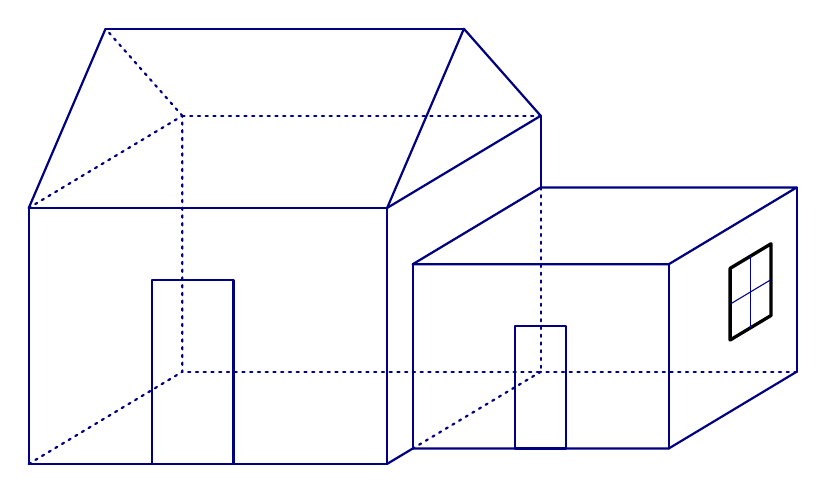
\begin{tikzpicture}[line cap=round, line join=round, x={(-0.5cm,-0.3cm)}, y={(1cm,0cm)}, z={(0cm,1cm)}, scale=1.3]
			\coordinate (A0) at (0,0,0);
			\coordinate (A1) at (3,0,0);
			\coordinate (A2) at (3,3.5,0);
			\coordinate (A3) at (0,3.5,0);
			\coordinate (B0) at (0,0,2.5);
			\coordinate (B1) at (3,0,2.5);
			\coordinate (B2) at (3,3.5,2.5);
			\coordinate (B3) at (0,3.5,2.5);
			\coordinate (R1) at (1.5,0,3.8);
			\coordinate (R2) at (1.5,3.5,3.8);
			\coordinate (C0) at (0,3.5,0);
			\coordinate (C1) at (2.5,3.5,0);
			\coordinate (C2) at (2.5,6,0);
			\coordinate (C3) at (0,6,0);
			\coordinate (D0) at (0,3.5,1.8);
			\coordinate (D1) at (2.5,3.5,1.8);
			\coordinate (D2) at (2.5,6,1.8);
			\coordinate (D3) at (0,6,1.8);
			\coordinate (W1) at (0.5, 6, 0.7);
			\coordinate (W2) at (1.3, 6, 0.7);
			\coordinate (W3) at (1.3, 6, 1.4);
			\coordinate (W4) at (0.5, 6, 1.4);
			\coordinate (P1) at (3, 1.2, 0);
			\coordinate (P2) at (3, 2.0, 0);
			\coordinate (P3) at (3, 2.0, 1.8);
			\coordinate (P4) at (3, 1.2, 1.8);
			\coordinate (AP1) at (2.5, 4.5, 0);
			\coordinate (AP2) at (2.5, 5.0, 0);
			\coordinate (AP3) at (2.5, 5.0, 1.2);
			\coordinate (AP4) at (2.5, 4.5, 1.2);
			\draw[blue!50!black, thick, dotted] (A1) -- (A0) -- (B0) -- (B1);
			\draw[blue!50!black, thick] (A1) -- (B1);
			\draw[blue!50!black, thick] (A1) -- (A2) -- (B2) -- (B1);
			\draw[blue!50!black, thick, dotted] (B0) -- (B3);
			\draw[blue!50!black, thick, dotted] (D0) -- (A3) -- (A0);
			\draw[blue!50!black, thick] (B2) -- (B3);
			\draw[blue!50!black, thick] (D0) -- (B3);
			\draw[blue!50!black, thick] (A2) -- (C1);
			\draw[blue!50!black, thick, dotted] (A3) -- (C1);
			\draw[blue!50!black, thick, dotted] (B0) -- (R1);
			\draw[blue!50!black, thick] (R1) -- (B1);
			\draw[blue!50!black, thick] (B3) -- (R2) -- (B2);
			\draw[blue!50!black, thick] (R1) -- (R2);
			\draw[blue!50!black, thick] (C1) -- (C2) -- (C3);
			\draw[blue!50!black, thick, dotted] (C3) -- (C0);
			\draw[blue!50!black, thick] (D0) -- (D1) -- (D2) -- (D3) -- cycle;
			\draw[blue!50!black, thick] (C1) -- (D1);
			\draw[blue!50!black, thick] (C2) -- (D2);
			\draw[blue!50!black, thick] (C3) -- (D3);
			\draw[black, very thick] (W1) -- (W2) -- (W3) -- (W4) -- cycle;
			\draw[blue!50!black, thin] (0.9, 6, 0.7) -- (0.9, 6, 1.4);
			\coordinate (W5) at (0.5, 6, 1.05);
			\coordinate (W6) at (1.3, 6, 1.05);
			\draw[blue!50!black, thin] (W5) -- (W6);
			\draw[blue!50!black, thick] (P1) -- (P2) -- (P3) -- (P4) -- cycle;
			\draw[blue!50!black, thick] (AP1) -- (AP2) -- (AP3) -- (AP4) -- cycle;
		\end{tikzpicture}
	\end{center}
\end{ex}

\begin{prop}[Propriétés d'une projection parallèle]
	\nline
	\begin{itemize}
		\item Une projection parallèle \textbf{conserve} les milieux, les contacts et les rapports de longueurs (pour des segments portés par une même droite ou par des droites parallèles, non parallèles à la direction de projection).
		\item Elle \textbf{ne conserve pas} les longueurs ni les angles.
	\end{itemize}
\end{prop}

\begin{rem}
	Les figures de ce chapitre sont dessinées en perspective cavalière.

	Ainsi, un angle droit n'est en général pas représenté par un angle droit, et deux segments de même longueur peuvent être représentés par des segments de longueurs différentes.

	En revanche, le milieu d'un segment est représenté par le milieu du segment qui le représente : c'est ce qui permet de placer les milieux $I$, $J$ et $K$ sur la figure de la pyramide.
\end{rem}

\begin{rem}
	La perspective cavalière n'est qu'une des façons de représenter l'espace sur une feuille : elle a l'avantage de la simplicité, mais elle déforme les longueurs selon la profondeur.

	Une autre méthode, plus fidèle à ce que perçoit l'œil, est la \textbf{perspective à points de fuite}, où les droites parallèles qui s'éloignent semblent converger vers un ou plusieurs points situés sur l'horizon selon l'orientation de l'objet, on parle de \textbf{perspective à un, deux ou trois points de fuite}, et c'est elle qui donne cette impression de relief et de profondeur si naturelle.

	\begin{center}
		\begin{tikzpicture}[line cap=round, line join=round, x=0.8cm, y=0.8cm]
			\coordinate (P1) at (0,0);
			\coordinate (P2) at (14,0);
			\coordinate (Av) at (9,-5);
			\coordinate (Ah) at (9,-2);
			\coordinate (Bg)  at (6,-4/3);
			\coordinate (Bgb) at (6,-10/3);
			\coordinate (Bd)  at (12,-2);
			\coordinate (Bdt) at (12,-0.8);
			\coordinate (Ct) at (10,-2/3);
			\draw [thick] (-2,0) -- (16,0);
			\draw [thick, dashed] (P1) -- (Bg);
			\draw [thick, dashed] (P1) -- (Bgb);
			\draw [thick, dashed] (P1) -- (Ct);
			\draw [thick, dashed] (P2) -- (Bd);
			\draw [thick, dashed] (P2) -- (Bdt);
			\draw [thick, dashed] (P2) -- (Ct);
			\fill [bleu!15]  (Ah) -- (Bg)  -- (Bgb) -- (Av) -- cycle;
			\fill [bleu!30]  (Ah) -- (Bdt) -- (Bd)  -- (Av) -- cycle;
			\fill [bleu!50]  (Ah) -- (Bg)  -- (Ct)  -- (Bdt) -- cycle;
			\draw [thick] (Av) -- (Ah);
			\draw [thick] (Bg) -- (Bgb);
			\draw [thick] (Bdt) -- (Bd);
			\draw [thick] (Ah) -- (Bg);
			\draw [thick] (Bgb) -- (Av);
			\draw [thick] (Av) -- (Bd);
			\draw [thick] (Ah) -- (Bdt);
			\draw [thick] (Bg) -- (Ct);
			\draw [thick] (Ct) -- (Bdt);
			\foreach \p in {P1,P2,Av,Ah,Bg,Bgb,Bd,Bdt,Ct}
			\fill (\p) circle (2pt);
			\node[anchor=south east] at (P1) {$P_1$};
			\node[anchor=south west] at (P2) {$P_2$};
		\end{tikzpicture}
	\end{center}
\end{rem}

